\begin{activity} \label{A:3.1.3}  
Consider the family of functions given by $h(x) = x^2 + \cos(kx)$, where $k$ is an arbitrary positive real number.
	\ba
	  \item Use a graphing utility to sketch the graph of $h$ for several different $k$-values, including $k = 1,3,5,10$.  Plot $h(x) = x^2 + \cos(3x)$ on the axes provided below.  
\begin{figure}[h]
\begin{center}
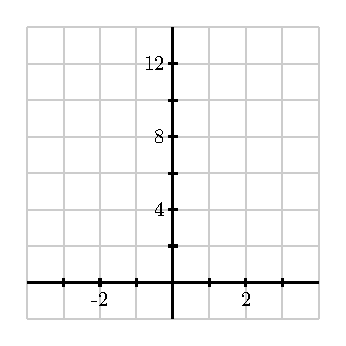
\includegraphics{figures/3_1_Act3.eps} 
\end{center}
\caption{Axes for plotting $y = h(x)$.} \label{F:3.1.Act3}
\end{figure}
	  What is the smallest value of $k$ at which you think you can see (just by looking at the graph) at least one inflection point on the graph of $h$?
	  \item Explain why the graph of $h$ has no inflection points if $k \le \sqrt{2}$, but infinitely many inflection points if $k > \sqrt{2}$.
	  \item Explain why, no matter the value of $k$, $h$ can only have a finite number of critical values.
	\ea
\end{activity}
\begin{smallhint}
	\ba
		\item Be sure to try some values between 1.5 and 2.
		\item Treat $k$ as an arbitrary constant in computing $h'(x)$ and $h''(x)$.  
		\item What is the largest value of $k\sin(kx)$?  How many times can $y = k\sin(kx)$ intersect the line $y = 2x$?
	\ea
\end{smallhint}
\begin{bighint}
	\ba
		\item Be sure to try some values between 1.5 and 2.  Remember that an inflection point is a point where concavity changes.
		\item Treat $k$ as an arbitrary constant in computing $h'(x)$ and $h''(x)$.  In particular, note that $h'(x) = 2x - k\sin(kx)$.
		\item Explain why $-k \le k\sin(kx) \le k$.  How many times can $y = k\sin(kx)$ intersect the line $y = 2x$?
	\ea
\end{bighint}
\begin{activitySolution}
	\ba
		\item In the graph below,
\begin{center}
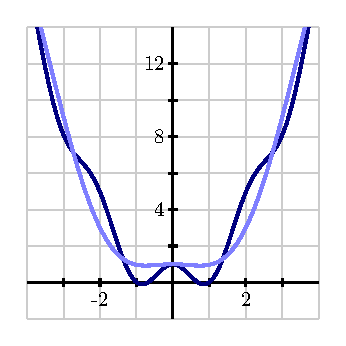
\includegraphics{figures/3_1_Act3Soln.eps} 
\end{center}
$h(x) = x^2 + \cos(3x)$ is given in dark blue, while $h(x) = x^2 + \cos(1.6x)$ is shown in light blue.  Close inspection of the light blue graph reveals some subtle changes in concavity around $x \approx \pm 0.5$.  For values smaller than $1.6$, it is very hard to visually detect any inflection points in $h(x)$.		
		\item Treating $k$ as an arbitrary constant, we first observe that $h'(x) = 2x - k\sin(kx)$. Again treating $k$ as a constant and differentiating, we find
		$$h''(x) = 2 - k^2\cos(kx).$$
		We seek the values of $x$ for which $h''(x) = 0$ at which $h''$ changes sign.  Setting $h''(x) = 0$ and rearranging the resulting equation, we now seek $x$ such that 
		$$k^2 \cos(kx) = 2,$$
		or
		$$\cos(kx) = \frac{2}{k^2}.$$
		Now, remember that $k$ is an arbitrary positive constant and recall that $-1 \le \cos(\theta) \le 1$ for all input values $\theta$.  If $\frac{2}{k^2} > 1$, then the equation $\cos(kx) = \frac{2}{k^2}$ has no solution.  Hence, whenever $k^2 < 2$, or $k < \sqrt{2} \approx 1.414$, it follows that the equation $\cos(kx) = \frac{2}{k^2}$ has no solutions $x$, which means that $h''(x)$ is never zero (indeed, for these $k$-values, $h''(x)$ is always positive so that $h$ is always concave up).
		
On the other hand, if $k \ge \sqrt{2}$, then $\frac{2}{k^2} \le 1$, which guarantees that $\cos(kx) = \frac{2}{k^2}$ has infinitely many solutions, due to the periodicity of the cosine function.  At each such point, $h''(x) = 2 - k^2 \cos(kx)$ changes sign, and therefore $h$ has infinitely many inflection points whenever $k \ge \sqrt{2}$.	 
		\item To see why $h$ can only have a finite number of critical values regardless of the value of $k$, consider the equation
		$$0 = h'(x) = 2x - k\sin(kx),$$
		which implies that $2x = k\sin(kx)$.  Since $-1 \le \sin(kx) \le 1$, we know that $-k \le k\sin(kx) \le k$.  Once $|x|$ is sufficiently large, we are guaranteed that $|2x| > k$, which means that for large $x$, $2x$ and $k\sin(kx)$ cannot intersect.   Moreover, for relatively small values of $x$, the functions $2x$ and $k\sin(kx)$ can only intersect finitely many times since $k\sin(kx)$ oscillates a finite number of times.  This is why $h$ can only have a finite number of critical values, regardless of the value of $k$.
	\ea
\end{activitySolution}
\aftera